\subsubsection{Teste da hipótese 2: Uma Análise Decomposta do Efeito do Lobby}

A avaliação da Hipótese 2, que postula uma maior influência das empresas sobre a atividade parlamentar em comparação com outros atores, exige uma análise que transcenda a simples contagem de reuniões. Uma análise preliminar do efeito marginal por reunião, apresentada na Figura \ref{fig:effect_linear_ppml_treatments}, sugere que as \acrshort{ong}s, paradoxalmente, exercem uma influência maior por encontro. Este resultado, embora contraintuitivo, destaca a necessidade de um modelo mais completo que considere a heterogeneidade dos atores de lobby.

\begin{figure}[htbp]
    \centering
    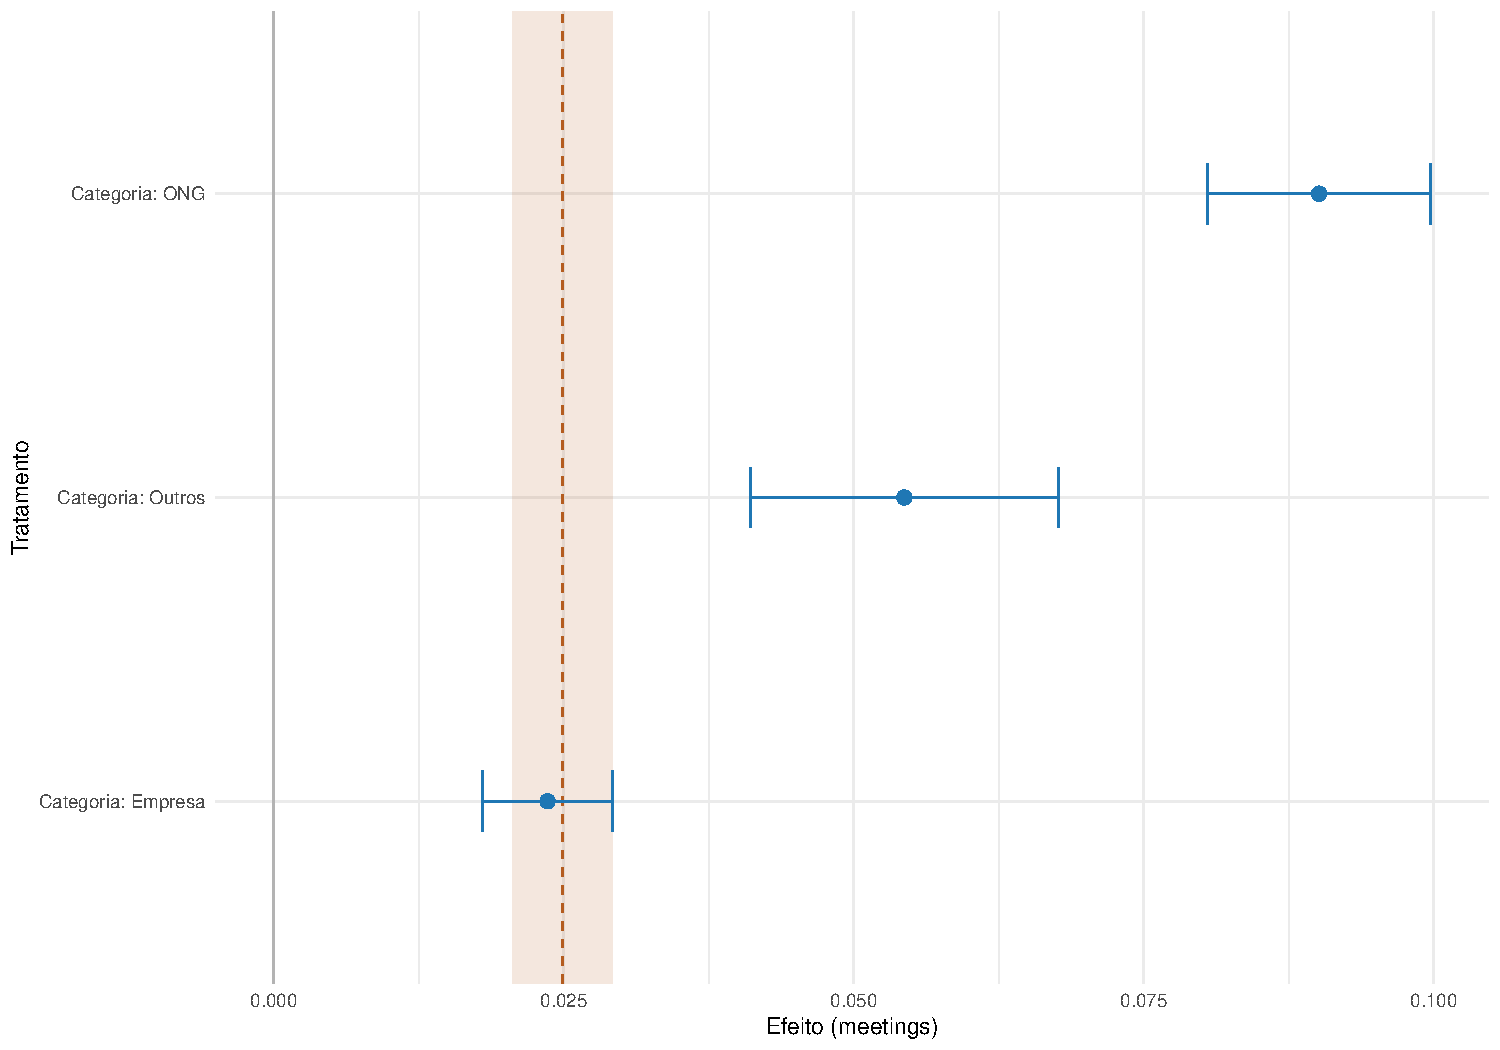
\includegraphics[width=\textwidth]{figures/h2_test/fig_coeff_treatments_overall.pdf}
    \caption{Efeito marginal por tipo de ator: especificação \acrshort{ppml}}
    \label{fig:effect_linear_ppml_treatments}
    \note{Cada ponto representa a estimativa do coeficiente para \textit{meetings}, associado a um tipo de ator (tratamento), refletindo o efeito marginal esperado de uma única reunião sobre o número de perguntas parlamentares, mantendo os efeitos fixos constantes. As linhas horizontais indicam os intervalos de confiança de 95\%. A faixa vertical sombreada representa o intervalo de confiança do efeito médio geral, servindo como referência.}
\end{figure}

O efeito marginal isolado, contudo, é insuficiente para um teste robusto da hipótese. A influência total de um grupo de interesse não depende apenas da \textit{eficácia} de cada reunião, mas também da sua capacidade de assegurar \textit{acesso} -- isto é, o volume de reuniões que consegue realizar. Argumentamos que o impacto total é uma função dessas duas componentes: a frequência do acesso e a eficácia da persuasão em cada encontro.

Para capturar essa dualidade, adotamos uma estratégia de modelagem em duas etapas que decompõe o processo de lobby da seguinte forma:
\begin{itemize}
    \item \textbf{Persuasão (Eficácia):} O processo pelo qual um lobista utiliza uma reunião para influenciar a atividade de um \acrshort{mpe}. Esta etapa, modelada com \acrshort{ppml}, responde à pergunta: \textit{"Quão eficaz é uma única reunião para gerar atividade parlamentar?"}
    \item \textbf{Acesso (Frequência):} O processo pelo qual um lobista garante reuniões com os \acrshort{mpe}s. Esta etapa, modelada com uma regressão Binomial Negativa, responde à pergunta: \textit{"Quantas reuniões um determinado lobista consegue obter?"}
\end{itemize}

Esta abordagem permite-nos decompor e compreender os mecanismos através dos quais diferentes atores exercem influência.

Para estimar o volume de reuniões (Acesso) - Etapa 1 -, utilizamos um modelo de regressão Binomial Negativo, apropriado para dados de contagem com sobredispersão. A variável dependente é o número de reuniões que um lobista realiza, e as variáveis explicativas incluem o orçamento de lobby, a categoria do ator (\acrshort{ong}, Empresa, Outros) e um termo de interação entre orçamento e categoria, além de controlos setoriais e geográficos. Os resultados completos são apresentados na Tabela \ref{tab:meetings_nb_centered}.

O coeficiente de interação entre ser uma empresa e o orçamento de lobby é particularmente revelador. Um resultado positivo e estatisticamente significativo para este termo indica que as empresas não só tendem a realizar mais reuniões em média, mas também demonstram uma "eficiência alocativa" superior: cada aumento percentual no seu orçamento se traduz num aumento maior no número de reuniões em comparação com as \acrshort{ong}s. A Figura \ref{fig:h2_pred_meetings} ilustra essa dinâmica, mostrando o número esperado de reuniões em função do orçamento.

\begin{figure}[htbp]
    \centering
    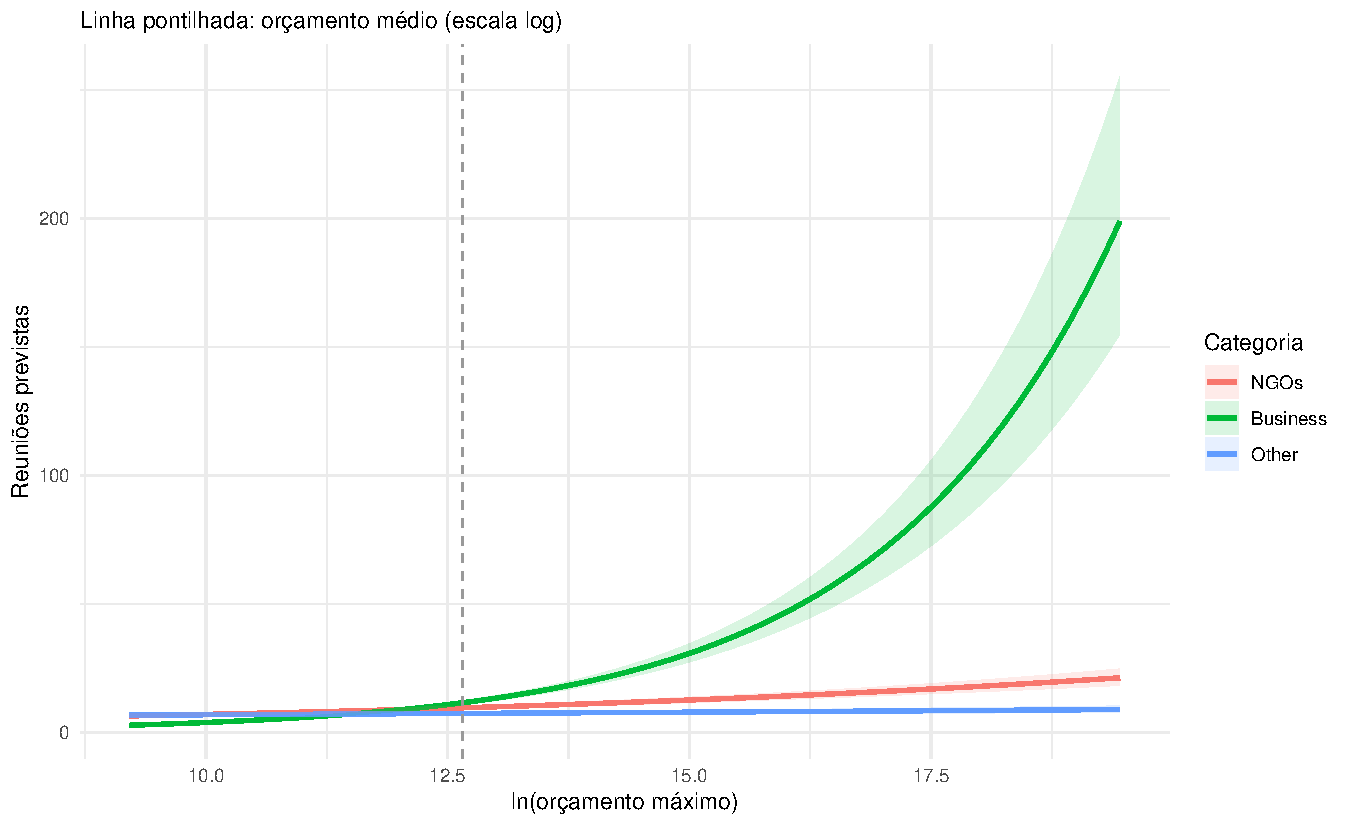
\includegraphics[width=\textwidth]{figures/h2_test/fig_pred_meetings_vs_budget_centered_by_category.pdf}
    \caption{Previsão do número de reuniões por categoria e orçamento}
    \label{fig:h2_pred_meetings}
    \note{O gráfico exibe o número esperado de reuniões (eixo Y) em função do logaritmo do orçamento de lobby (eixo X), com base no modelo Binomial Negativo. As curvas representam a previsão para cada categoria de ator, mantendo as demais variáveis em seus valores médios ou modais. A linha tracejada vertical indica o orçamento médio na amostra. As áreas sombreadas correspondem aos intervalos de confiança de 95\%.}
\end{figure}

Observa-se um ponto de inflexão: abaixo de um orçamento de aproximadamente \$27.000 ($\approx e^{10.2}$), as \acrshort{ong}s tendem a realizar mais reuniões. Acima desse limiar, a capacidade das empresas de converter recursos financeiros em acesso torna-se proeminente, e a disparidade cresce exponencialmente com o orçamento.

Para estimar o efeito agregado (Etapa 2), combinamos os resultados das duas etapas, multiplicando o número esperado de reuniões (o \textit{Acesso}, da Etapa 1) pelo efeito marginal por reunião (a \textit{Persuasão}, da Figura \ref{fig:effect_linear_ppml_treatments}) para cada categoria de ator e nível de orçamento. O resultado, ilustrado na Figura \ref{fig:h2_total_effects}, representa uma aproximação de primeira ordem do impacto total do lobby.

\begin{figure}[htbp]
    \centering
    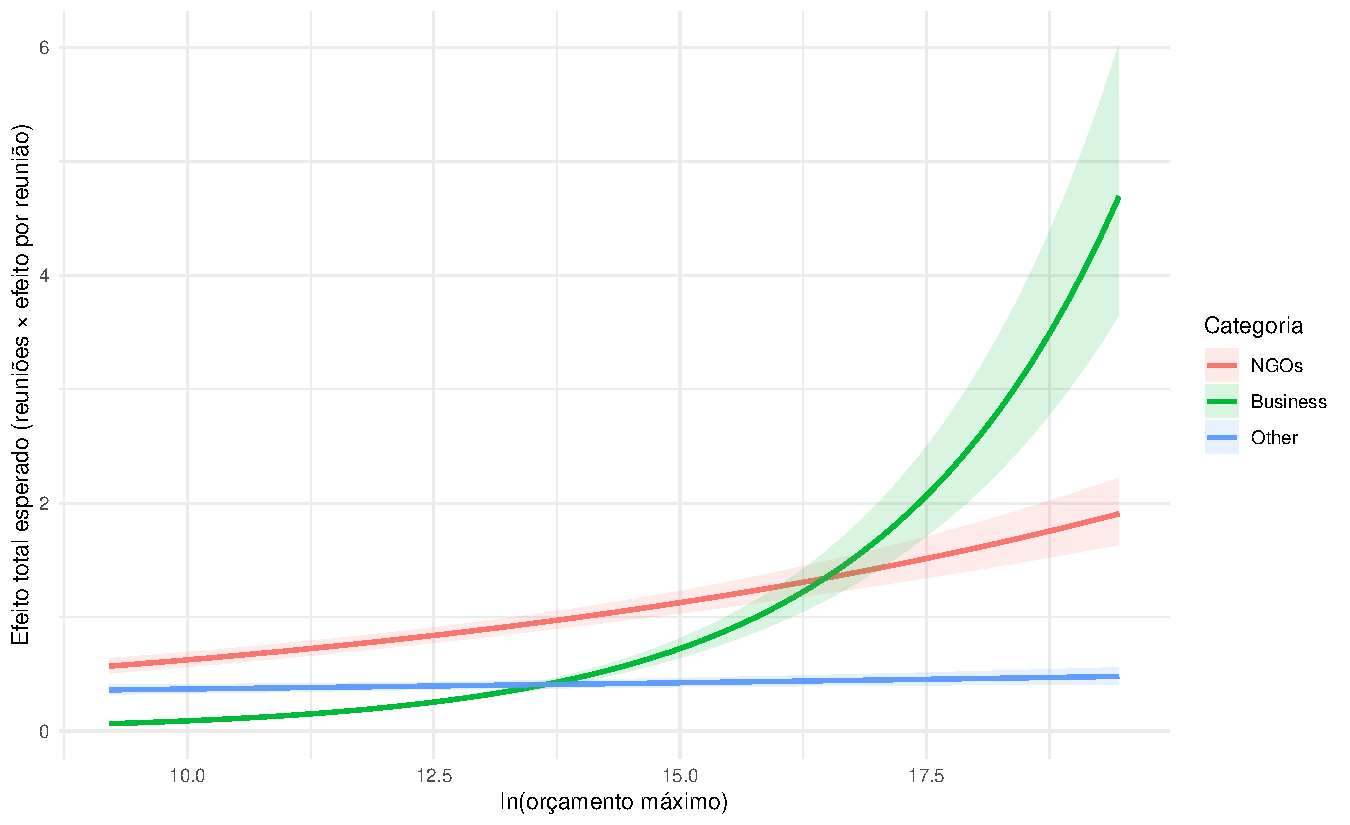
\includegraphics[width=\textwidth]{figures/h2_test/fig_total_effect_vs_budget_by_category.pdf}
    \caption{Efeito total estimado por categoria e orçamento}
    \label{fig:h2_total_effects}
    \note{O gráfico representa o efeito total esperado, calculado como o produto do número previsto de reuniões (da Figura \ref{fig:h2_pred_meetings}) e do coeficiente de efeito marginal por reunião (da Figura \ref{fig:effect_linear_ppml_treatments}). O eixo Y representa o aumento esperado no número de perguntas parlamentares.}
\end{figure}

A análise do efeito total revela uma relação complexa e não-linear. Embora uma única reunião com uma \acrshort{ong} seja, em média, mais influente, a superioridade das empresas em garantir um grande volume de acesso, especialmente quando dispõem de orçamentos elevados, reverte essa vantagem. Para orçamentos abaixo de \$8,8 milhões ($\approx e^{16}$), o efeito total das \acrshort{ong}s permanece superior. No entanto, acima de \$40 milhões ($\approx e^{17.5}$), o efeito agregado das empresas torna-se substancialmente maior.

Estes resultados oferecem um suporte nuançado à Hipótese 2 e dialogam diretamente com a literatura sobre os mecanismos de influência do lobby. A influência das empresas não é incondicionalmente superior, mas torna-se dominante quando alavancada por vastos recursos financeiros, um achado que se alinha com a discussão sobre a desigualdade de representação \cite{mahoney_lobbying_2007}. A decomposição do efeito em "acesso" e "persuasão" permite-nos explorar as diferentes naturezas dos recursos mobilizados pelos atores, conforme aponta a literatura \cite{de_figueiredo_advancing_2014, Pop2013Lobbying}.

A maior eficácia marginal por reunião das \acrshort{ong}s pode ser interpretada à luz do seu capital reputacional e da sua legitimidade percebida \cite{bunea2018legitimacy}. Do ponto de vista do comportamento parlamentar, interagir com \acrshort{ong}s pode ser uma estratégia de \textit{vote-seeking} para os \acrshort{mpe}s, que buscam sinalizar alinhamento com causas de interesse público e, assim, aumentar seu apelo eleitoral \cite{Ibenskas2021, mayhew2004congress}.

Por outro lado, a capacidade das grandes corporações de converter recursos financeiros em um volume massivo de acesso aponta para outro mecanismo de influência: a subsidiação de informação. Para atingir seus objetivos de carreira (\textit{career-seeking}) e de formulação de políticas (\textit{policy-seeking}), os parlamentares necessitam de informação técnica e especializada \cite{daniel2015career, kluver_informational_2012}. As grandes empresas, com seus recursos, estão em posição privilegiada para fornecer este subsídio informacional, estabelecendo uma relação de troca \cite{huwyler_no_2023} que lhes garante um acesso privilegiado e contínuo. Assim, a capacidade de "saturar" o ambiente informacional com interações frequentes parece ser um fator decisivo para a sua influência agregada.

É importante notar que esta abordagem metodológica assenta na premissa de \textit{separabilidade} entre os processos de "acesso" e "persuasão". Esta premissa implica que, após controlarmos pelas variáveis observáveis (como o orçamento), os fatores não observados que tornam um lobista eficaz em garantir reuniões são estatisticamente independentes dos fatores não observados que o tornam influente durante essas reuniões. A suposição de separabilidade poderia ser violada se, por exemplo, uma "qualidade" ou "reputação" intrínseca do lobista, não capturada pelo modelo, afetasse simultaneamente a sua capacidade de agendar reuniões e a recetividade dos parlamentares às suas propostas. Nesse cenário, a multiplicação dos efeitos poderia levar a uma estimativa enviesada do impacto total.

Em suma, os resultados indicam que, embora o discurso das \acrshort{ong}s possa ter maior ressonância por interação, a capacidade financeira das grandes empresas permite-lhes superar essa desvantagem através de uma presença quantitativamente esmagadora, confirmando a importância crítica dos recursos na determinação da influência política.